\begin{figure}[H]
	\centering
	\subfloat[\SI{30}{\volt} Source]{\label{fig:vSweep30}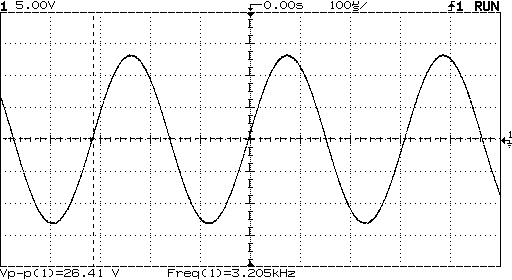
\includegraphics[width=.3\textwidth]{img/shot/pt4_30vShot.png}}
	\quad
	\subfloat[\SI{15}{\volt} Source]{\label{fig:vSweep15}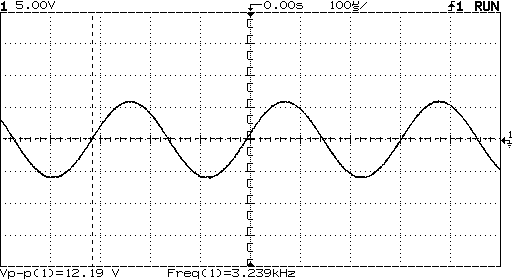
\includegraphics[width=.3\textwidth]{img/shot/pt4_15vShot.png}}
	\quad
	\subfloat[\SI{5}{\volt} Source]{\label{fig:vSweep5}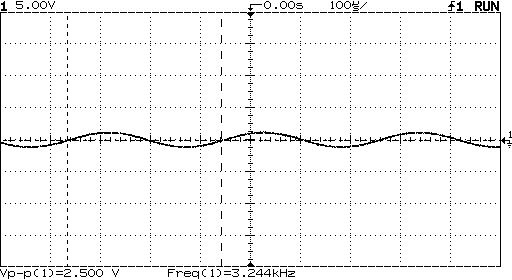
\includegraphics[width=.3\textwidth]{img/shot/pt4_5vShot.png}}

	\parbox{.9\textwidth}{
	\caption[Oscilloscope Screenshots --- Voltage Sweep]{Oscilloscope
	screenshots for the performed voltage sweep.  Note that while the output
	frequency remains roughly constant, the peak-to-peak voltage of the signal
	decreases with decreasing source voltage.}
	\label{fig:vSweepPlots}}
\end{figure}

\begin{figure}[H]
	\centering
	\subfloat[\SI{100}{\kilo\ohm} Load]{\label{fig:rSweep100k}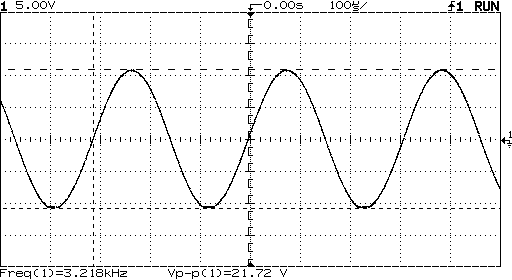
\includegraphics[width=.3\textwidth]{img/shot/pt5_100kShot.png}}
	\quad
	\subfloat[\SI{10}{\kilo\ohm} Load] {\label{fig:rSweep10k} 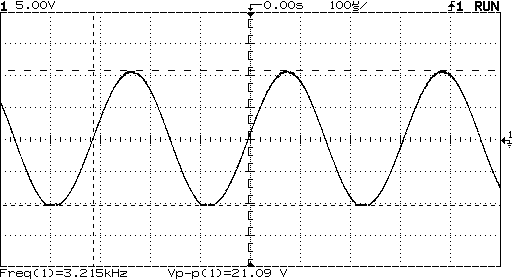
\includegraphics[width=.3\textwidth]{img/shot/pt5_10kShot.png}}
	\quad
	\subfloat[\SI{1}{\kilo\ohm} Load]  {\label{fig:rSweep1k}  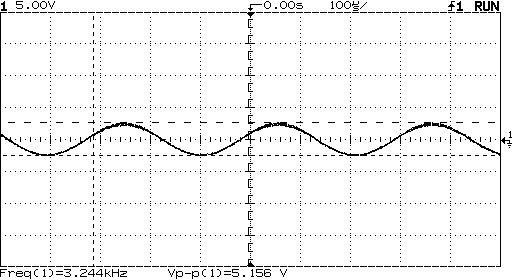
\includegraphics[width=.3\textwidth]{img/shot/pt5_1kShot.png}}

	\parbox{.9\textwidth}{
	\caption[OScilloscope Screenshots --- Resistance Sweep]{Screenshots
	captured from the oscilloscope while varying the load resistance.  Like the
	voltage sweep shown in Figure~\ref{fig:vSweepPlots}, the output voltage
	decreases while the frequency remains roughly constant.}
	\label{fig:rSweepPlots}}
\end{figure}
